\documentclass[final,leqno,onefignum,onetabnum]{siamltex1213bueler}
% siamltex1213bueler.cls is a two or three line change of siamltex1213.cls to permit
% pdflatex to work and not spew warnings

\usepackage{amssymb,amsmath}

\usepackage{times}

%\theoremstyle{definition}
\newtheorem{example}{Example}

% math macros
\newcommand\bb{\mathbf{b}}
\newcommand\bbf{\mathbf{f}}
\newcommand\bn{\mathbf{n}}
\newcommand\bq{\mathbf{q}}
\newcommand\bu{\mathbf{u}}
\newcommand\bv{\mathbf{v}}
\newcommand\by{\mathbf{y}}

\newcommand\bQ{\mathbf{Q}}
\newcommand\bV{\mathbf{V}}
\newcommand\bX{\mathbf{X}}

\newcommand\CC{\mathbb{C}}
\newcommand{\DDt}[1]{\ensuremath{\frac{d #1}{d t}}}
\newcommand{\ddt}[1]{\ensuremath{\frac{\partial #1}{\partial t}}}
\newcommand{\ddx}[1]{\ensuremath{\frac{\partial #1}{\partial x}}}
\newcommand{\ddy}[1]{\ensuremath{\frac{\partial #1}{\partial y}}}
\newcommand{\ddxp}[1]{\ensuremath{\frac{\partial #1}{\partial x'}}}
\newcommand{\ddz}[1]{\ensuremath{\frac{\partial #1}{\partial z}}}
\newcommand{\ddxx}[1]{\ensuremath{\frac{\partial^2 #1}{\partial x^2}}}
\newcommand{\ddyy}[1]{\ensuremath{\frac{\partial^2 #1}{\partial y^2}}}
\newcommand{\ddxy}[1]{\ensuremath{\frac{\partial^2 #1}{\partial x \partial y}}}
\newcommand{\ddzz}[1]{\ensuremath{\frac{\partial^2 #1}{\partial z^2}}}
\newcommand{\Div}{\nabla\cdot}
\newcommand\eps{\epsilon}
\renewcommand{\grad}{\nabla}
\newcommand{\ihat}{\mathbf{i}}
\newcommand{\ip}[2]{\ensuremath{\left<#1,#2\right>}}
\newcommand{\jhat}{\mathbf{j}}
\newcommand{\khat}{\mathbf{k}}
\newcommand{\nhat}{\mathbf{n}}
\newcommand\lam{\lambda}
\newcommand\lap{\triangle}
\newcommand\Matlab{\textsc{Matlab}\xspace}
\newcommand\RR{\mathbb{R}}
\newcommand\vf{\varphi}


\title{Conservation for fluid layers with free boundaries\thanks{Draft date: \today.  Supported by NASA grant \# NNX13AM16G.}} 

\author{Ed Bueler\thanks{Dept.~of Mathematics and Statistics, and Geophysical Institute, University of Alaska Fairbanks (\texttt{elbueler@alaska.edu}).}}

\begin{document}
\maketitle
\slugger{siap}{xxxx}{xx}{x}{x--x}

\begin{abstract}
FIXME
\end{abstract}


\pagestyle{myheadings}
\thispagestyle{plain}
\markboth{ED BUELER}{CONSERVATION FOR FLUID LAYERS WITH FREE-BOUNDARIES}


\section{Introduction}  \label{sec:intro}

Consider a fluid which moves in a thin layer over a substrate.  Fluid mass can be added or removed at the boundary of the three-dimensional fluid by processes like precipitation, evaporation, ablation, and so on.  Fluid can even be added/removed by phase change if we define the fluid region as being only a single phase.  Through both flow and such boundary sources, the substrate area covered by the fluid changes in time.  A balance of precipitation and flow can extend the fluid-covered region, or a balance of flow and ablation can reduce the region or even remove the layer entirely.

We will only consider models which describe such fluid layers by a \emph{thickness}, or equivalent quantity, typically by integrating vertically (e.g.~along gravity).  In such models the boundary addition/removal processes become signed source terms in a two-spatial-dimension conservation equation.  The layer occupies a subset of a larger fixed region of the plane, and the domain where the fluid layer is present, and the conservation equation applies, is the set where the thickness is positive.  This domain changes in time, so the conservation problem is of free-boundary type.

In such layer models for constant density fluids the thickness is the conserved quantity, equivalent to mass, and this thickness must be nonnegative.  In layer models for variable density fluids the vertical integral of density is the conserved quantity, and it must be nonnegative.  In layer models of conservation of energy, the vertical integral of internal energy or temperature is the conserved quantity, and in some such cases this vertical energy must be bounded below because the layer is only one phase \cite{AschwandenBuelerKhroulevBlatter}.  However, we consider only conservation of scalar properties, and not, for example conservation of vectors like momentum.  As the mass of a constant-density fluid is a primary example of the conserved scalar in such layer models, we will for simplicity call the conserved quantity ``mass'' and the corresponding nonnegative variable ``thickness''.

Thus we suppose $\Omega \subset \RR^d$, $d\ge 1$, is a bounded open region with regular (Lipshitz) boundary.  Our time-dependent model is usually stated in strong form, combining a conservation equation and an oft-ignored constraint:
\begin{align}
u_t + \Div \bq &= f(u,x,t) &&\text{in } \Omega, \text{ where } u > 0 \label{eq:massconserve} \\
u &\ge 0 &&\text{in } \bar\Omega. \label{eq:constraint}
\end{align}
Note $u(x,t)$ is defined for all $x\in \bar\Omega$ and $t>0$, even where there is no fluid and $u(x,t)=0$.

The form of the flux $\bq$, that is, how it depends on the unknown $u$ or its gradient $\grad u$, is quite general here,
\begin{equation}
\bq = \bq(\grad u,u,x,t), \label{eq:fluxdepends}
\end{equation}
but with more detail below in subsection \ref{subsec:fluxassumptions}.

In fact our broader conclusions apply equally to models where $\bq$ depends \emph{globally} on the conserved quantity $u$ and its derivatives, perhaps through integrals but more likely through coupling to other variables and equations.  Such integro-differential or coupled models are exactly our interest, and the reader should think that while we focus only on the mass-conservation equation in such systems, we don't intend that this equation be decoupled.  However, so as to find rigorous and precise results here, we need to have some assurance of well-posedness at each time step (section \ref{sec:mono}), and so we mostly restrict to cases \eqref{eq:fluxdepends}.  An exception occurs in subsection FIXME, which covers an example where the form of $\bq$ involves a spatial integral.

Furthermore, in many examples we may think of the fluid moving at some vertically-averaged velocity $\bX=\bX(x,t)$ determined by ``external'' factors, and thus $\bq = \bX u$.  We address such cases in subsection FIXME.  The broader results we find there will apply equally if that velocity if actually a result of a coupled solution of a mass conservation plus momentum conservation system, for example, as long as the velocity field has the regularity we need to apply the theory (i.e.~as in subsection \ref{subsec:fluxassumptions}).

Constraint \eqref{eq:constraint} comes from the meaning of $u$ as a thickness, of course, and we say that the layer \emph{exists} where $u(x,t)>0$, and that it is \emph{absent} otherwise.  We emphasize that \emph{strong form} conservation equation \eqref{eq:massconserve} only applies where the layer exists.  Well-posedness of the combined problem \eqref{eq:massconserve}--\eqref{eq:constraint} requires a precise specification of admissible functions and a weak formulation (sections \ref{sec:weakform} and \ref{sec:mono}).

Fluid layer problems of the type addressed here appear within earth-system and climate models for the ice sheet, sea-ice, and even ocean components (Figure \ref{fig:climatepictures}).  Numerical approximations of these time-evolving fluid layer problems necessarily discretize time in some manner, and our analysis is based on this fact.  We semi-discretize the mass conservation equation in time by a one-step method and pose the single-time-step, continuous-space problem in weak variational form.  (Multi-stage but one step time-discretization methods, such as Runge-Kutta methods, are also allowed; see the Appendix.)  A broad selection of methods are possible when discretizing space to solve this single-time-step problem numerically, including finite difference/volume/element methods and even spectral methods, but, until section FIXME, our approach is independent of any chosen spatial discretization.

\begin{figure}[ht]
\begin{center}
FIGURE (FIXME)
%\includegraphics[width=2.0in,keepaspectratio=true]{domains-fig}
\end{center}
\caption{Time-stepping, free-boundary fluid layer mass conservation problems occur for several components of the earth-system and climate models, including ice sheet (a), sea ice (b), and ocean (c) components.}
\label{fig:climatepictures}
\end{figure}

In the time-semi-discretized case, each time-step requires the solution of a (continuous) free boundary problem in space.  Our first questions about such models is
  \begin{quote}
  \renewcommand{\labelenumi}{(\roman{enumi})}
  \begin{enumerate}
  \item \emph{Is the weakly-posed, single-time-step, free-boundary problem well-posed?}
  \end{enumerate}
  \end{quote}
The answer to (i) depends on the form of the flux, but we can show, by essentially-standard methods applied to the variational inequality form of the weakly-posed problem (section \ref{sec:mono}), that the answer is often ``yes''.

Our second question is perhaps less obvious, but of substantial importance in modeling practice:
  \begin{quote}
  \renewcommand{\labelenumi}{(\roman{enumi})}
  \begin{enumerate}
  \setcounter{enumi}{2}
  \item \emph{Can the modeled total mass of the fluid layer, inside its free boundary, be conserved exactly in the sense that a computable space-time integral of the source term $f$, over the time step, is equal to the change in total mass in that time step?}
  \end{enumerate}
  \end{quote}
By considering this question abstractly, we conclude that the answer is ``no,'' in particular in the case where the answer to (i) is ``yes.''  That is, our answer to the brief question ``can a numerical model of a fluid layer governed by \eqref{eq:massconserve} and \eqref{eq:constraint} conserve mass?'' is ``no''.  We can, however, quantify the non-conservation error associated to the free boundary (below).

Free-boundary problems of the above kind appear for the evolution of ice sheets \cite{BLKCB,CDDSV,EgholmNielsen2010,JouvetBueler2012}, shallow liquid water flowing over marshes \cite{AlonsoSantillanaDawson}, shallow water equation models for tsunumi run-up \cite{LeVequeGeorge2008}, coupled surface/subsurface hydrological modelling \cite{Maxwelletal2014}, subglacial hydrology \cite{AschwandenBuelerKhroulevBlatter,BuelervanPeltDRAFT,Schoofetal2012}, supraglacial runoff \cite{AschwandenBuelerKhroulevBlatter}, ice shelves [FIXME], and sea ice [FIXME], among many other applications.  FIXME: point out categorization by diffusive versus hyperbolic

Theoretical guidance as to the degree of achievable numerical (i.e.~discrete) conservation is generally absent in the literature of free-boundary fluid problems.  For instance, within the context of glacier \cite{JaroschSchoofAnslow2013} and ice shelf \cite{Albrechtetal2011} modeling, schemes for improved discrete mass conservation at free boundaries are proposed, but this small literature provides only \emph{ad hoc} solutions to improve conservation at the discrete level.  \emph{Local} discrete conservation, within the fluid and away from the free boundary, is a common goal and property of numerical schemes \cite{LeVeque}.  Indeed when we consider spatial discretization near the end of the paper (section FIXME), we will simply \emph{assume} that such local discrete conservation is already exact.  The discrete conservation limitations we identify are thus entirely at the free boundary.  Regarding conservation issues, we focus on the advance of the fluid layer into areas where it was absent a time-step earlier, and on its retreat from areas where it was present a time-step earlier.

Climate-scale circulation models generally claims exact discrete conservation as a goal [FIXME: CITE], but apparently always in a context without free boundary.  Such climate models are ``multiphysics'' models which generally attempt to conserve masses of the phases of water (in particular) separately, as these phases have different physical properties relevant to earth system dynamics.  For example, snow and ice have higher albedo and lower density than the liquid ocean.  In many such models, one or more fluids or phases form a layer with a moving free boundary.  We believe that auditable mass conservation does not generally occur in that case, except perhaps through \emph{ad hoc} redistribution of mass, or \emph{ad hoc} discrete schemes to locally balance the books at the free boundary.  Discrete conservation is presumably recovered in the temporal and spatial refinement limit in such models.

In our work, the single time-step problem is put in weak form, specifically a variational inequality (section \ref{sec:weakform}).  The nonnegativity of the thickness, $u\ge 0$, is a constraint which determines a closed, convex subset of a Banach space, the set of admissible thickness functions.  The constraint is active when negativity of the combined terms $f - \Div \bq$ in \eqref{eq:massconserve} would send the thickness below zero.  Maximum principles for the higher-order terms $\Div\bq$ in \eqref{eq:massconserve}, if applicable at all, play no role because they cannot maintain the constraint when $f<0$.  Though the form of the flux certainly affects the well-posedness, stability, and approximate-ability of the single time-step problem, our conclusions about conservation corrections at the free boundary are insensitive to the form or provenance of the flux $\bq$.

We identify the ``retreat area'' during the time step as fundamental.  By definition this is the region where the fluid layer thickness is positive at the beginning of the time step, and, through flow and boundary-source terms, the thickness is zero at the end of the time step.  That is, fluid was completely lost from the retreat area at some time during the time-step.  Even for well-behaved source terms (e.g.~smooth in time and space) and short time steps, the retreat area can be of essentially arbitrary size.  For example, in a varying climate a large area of thin ice sheet or sea ice can melt, or a large area of a layer of surface water on ground can evaporate, and so on, during one time step.

We then define the ``retreat loss'' $R_n$ as the change in mass, during the time step $[t_{n-1},t_n]$, within the retreat area.  In these terms we can answer our second question more precisely:
\begin{itemize}
\item  \emph{The retreat loss cannot be exactly balanced by a computable integrals of the source during the discrete time-step.}
\item  \emph{A time-stepping model which reports mass conservation quantities, so as to ``balance the books'' for the model user, should report a retreat loss time-series $\{R_n\}$, or equivalent quantity, additional to any integrals of the source terms.}
\end{itemize}
The details appear in section \ref{sec:timeseries}.  Note that the retreat losses $R_n$ becomes zero under temporal refinement only.

The above conclusions apply in the time-semi-discretized case and thus are independent of particular spatial discretization schemes.  However, in the case where the single time-step problem is well-posed in a sufficiently well-behaved Banach space (e.g.~in $W_0^{1,p}(\Omega)$; see sections \ref{sec:weakform} and \ref{sec:mono}), and if space is discretized using a scheme that allows a finite volume (cell-wise) mass conservation interpretation, we identify an additional, computable free-boundary-related conservation error.  This error $S_n$, which we call a ``shell error'' for convenience, occurs along that part of the free boundary where the flux goes to zero in the continuous case, generically has a nonzero value in the space-discretized case; see section FIXME for details.  In summary we can say,
\begin{itemize}
\item  \emph{A time- and space-discretized model should report, as a conservation error which goes to zero under spatial refinement only, an additional time-series $\{S_n\}$ which is the sum over the free boundary of the discrete flux, in cells where that flux would be zero in the continuous-space case.}
\end{itemize}
The shell errors $S_n$ go to zero under spatial refinement even when the time-step is not reduced.

With the conservation-correction time-series $\{R_n\}$ and $\{S_n\}$, a numerical model can ``balance the books'' exactly (i.e.~up to rounding error) in a manner which properly reflects the continuum model of the fluid layer.  A user of such models can adequately assess whether these free-boundary-related conservation errors are acceptably small, just in the way \emph{a posteriori} estimates are used to assess whether truncation errors are acceptably small.

We believe that avoidance of, or at least clearer understanding of, \emph{ad hoc} discrete schemes to maintain conservation at free boundaries will be easier once theoretical limits on discrete conservation are acknowledged, as here.  With the retreat loss correction, for example, when a large area of ice sheet or sea-ice is modeled as melting entirely in a climate simulation model, that model can measure the amount of non-conservation of the mass of water in each phase, even if that model simply uses the retreat loss as a mass transfer into the liquid phase.  More powerfully, adaptive time-stepping schemes can be modified to reduce this kind of conservation error, and adaptive mesh refinement or other paradigms can reduce the shell error (see above).  Climate models will, in any case, be able to more-accurately report uncertainty in important mass transfers between component fluids of the climate.



\section{Discrete-time formulation}  \label{sec:discreteform}

\subsection{Strong formulation of the single time-step problem}  \label{subsec:strongsingle}  To construct the time-semi-discretized problem, let $T>0$ and let $\{t_n\}_{n=0}^N$ be a sequence of increasing times on $[0,T]$ with $t_0=0$ and $t_N=T$.  The single time-step problem determines a new thickness function $u_n(x) \approx u(x,t_n)$ given the old value $u_{n-1}(x) \approx u(x,t_{n-1})$ (Figure \ref{fig:timestepcartoon}).

\begin{figure}[ht]
\begin{center}
% this one is generated by figs1d.py in layer-conserve/talks/
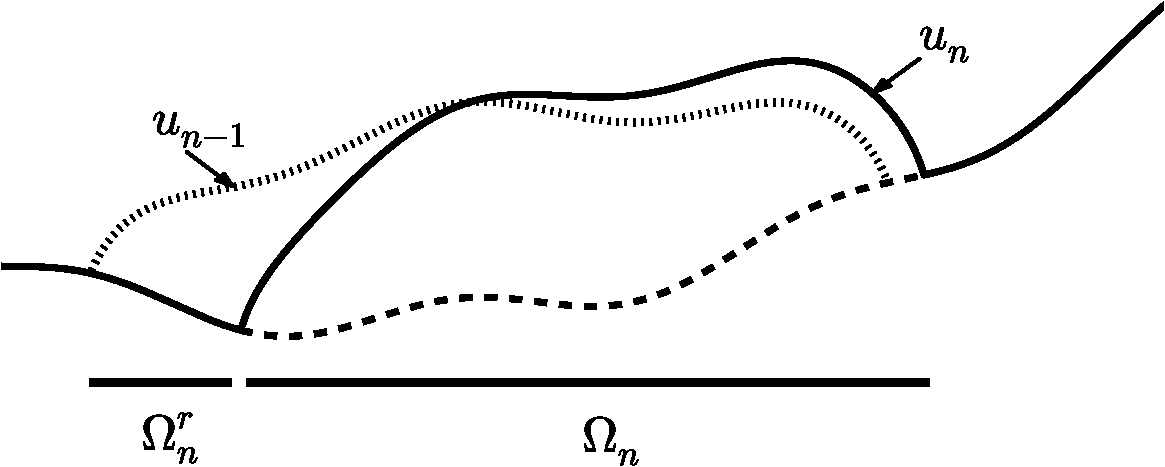
\includegraphics[width=3.9in,keepaspectratio=true]{time-step-cartoon}
\end{center}
\caption{The single time-step problem is a free boundary problem determining a new layer thickness $u_n$ from an old thickness $u_{n-1}$.}
\label{fig:timestepcartoon}
\end{figure}

Corresponding to \eqref{eq:massconserve} and \eqref{eq:constraint}, the strong form of the problem is
\begin{align}
\frac{u_n - u_{n-1}}{\Delta t} + \Div \bQ_n(\grad u_n,u_n,x) &= F_n(u_n,x) &&\text{in } \Omega, \text{ where } u_n > 0 \label{eq:semimassconserve} \\
u_n &\ge 0 &&\text{in } \overline{\Omega} \label{eq:semiconstraint}
\end{align}
In equations \eqref{eq:semimassconserve}--\eqref{eq:semiconstraint}, the semi-discretization procedure applied to \eqref{eq:massconserve} and \eqref{eq:constraint} generates the key functions
\begin{equation}
\bQ_n(\bX,v,x), \quad F_n(v,x) \label{eq:functionalforms}
\end{equation}
Here $\bX\in\RR^d$ is any vector, $v\in\RR$, and $x\in \Omega$.  We will assume $\bQ_n$ is defined for any $v\in\RR$, not just $v\ge 0$.  Furthermore, we assume $\bQ_n$ is defined for all $x\in\Omega$, not just where $v(x)>0$, but that $\bQ_n(\bX,0,x)=0$ because this is the model for a \emph{layer} mass flux (subsection \ref{subsec:fluxassumptions}).

The weak form of problem \eqref{eq:semimassconserve} and \eqref{eq:semiconstraint} is stated in section \ref{sec:weakform} with attention to function spaces and well-posedness.  Though the weak form is more fundamental, both tradition and the developed intuition of practitioners suggests we should state the strong form first.  Essentially all climate-relevant literature uses the strong form rather than weak variational statements of the full free-boundary problem.

In the simplest implicit time-discretized case, namely using a backward Euler scheme applied to \eqref{eq:massconserve}--\eqref{eq:constraint}, we have $\bQ_n = \bq(\bX,v,x,t_n)$ and $F_n = f(v,x,t_n)$.  However, according to the particular discretization procedure, the source function $F_n$ ``absorbs'' all the terms, whether evaluated at $t_{n-1}$ or $t_n$, which do not involve the flux $\bq$ evaluated at time $t_n$.

For example, and including the backward Euler case above, consider a $\theta$-method discretization of \eqref{eq:massconserve} with $0\le \theta \le 1$.  The result is
\begin{align}
  &\frac{u_n - u_{n-1}}{\Delta t} + \theta\, \Div \bq(\grad u_n,u_n,x,t_n) + (1-\theta) \Div \bq(\grad u_{n-1},u_{n-1},x,t_{n-1}) \label{eq:thetamethod} \\
  &\qquad =  \theta f(u_n,x,t_n) + (1-\theta) f(u_{n-1},x,t_{n-1}). \notag
\end{align}
This is of form \eqref{eq:semimassconserve} with
\begin{align*}
\bQ_n(\bX,v,x) &= \theta\, \bq(\bX,v,x,t_n), \\
F_n(v,x)       &= \theta f(v,x,t_n) + (1-\theta) f(u_{n-1},x,t_{n-1}) \\
               &\qquad - (1-\theta) \Div \bq(\grad u_{n-1},u_{n-1},x,t_{n-1}),
\end{align*}
where the already-computed function $u_{n-1}(x)$ represents part of the dependence on $x$.  The $\theta=0$ case of \eqref{eq:thetamethod} is the forward Euler method, $\theta=1/2$ is trapezoid, and $\theta=1$ is backward Euler.  The fact that $\bQ_n=0$ in the forward Euler method is included in our weakly-posed theory (subsection FIXME).  Naturally, however, implicitness is helpful for stability and thus efficiency reasons.

Our theory is not limited to the $\theta$-methods.  In particular, multi-stage one-step schemes like Runge-Kutta can be put in the form of \eqref{eq:semimassconserve}---see the Appendix.  There is every reason to expect multi-step integration methods to also fit into the given framework, but the low regularity of the solution in the vicinity of the free boundary suggests caution in any expected accuracy improvements from such schemes.

\subsection{Associated set decomposition}  \label{subsec:setdecompose}  We decompose $\Omega$ using the solution of problem \eqref{eq:semimassconserve} and \eqref{eq:semiconstraint}, defining three disjoint regions based on $u_n$ and $u_{n-1}$:
\begin{align*}
\Omega_n &= \left\{x \in \Omega \,\big|\, u_n(x)>0\right\}, \\
\Omega_n^r &= \left\{x \in \Omega \,\big|\, u_n(x)=0 \text{ and } u_{n-1}(x) > 0\right\}, \\
\Omega_n^0 &= \left\{x \in \Omega \,\big|\, u_n(x)=0 \text{ and } u_{n-1}(x) = 0\right\},
\end{align*}
so that
\begin{equation}
\Omega = \Omega_n \cup \Omega_n^r \cup \Omega_n^0.  \label{eq:omegadecomposition}
\end{equation}
Here the superscript ``$r$'' stands for ``retreat,''\footnote{A symmetry has been broken, as we could have decomposed $\Omega= \Omega_{n-1} \cup \Omega_n^a \cup \Omega_n^0$ where $\Omega_{n-1}$ is the support of $u_{n-1}$ and $\Omega_n^a = \{u_n(x) > 0 \text{ and } u_{n-1}(x) = 0\}$ is the ``advance'' set.  This alternate theory offers no apparent advantages or disadvantages.} and $\Omega_n^r$ is called the \emph{retreat set}.

Figure \ref{fig:domains} shows this decomposition of $\Omega$.  Note that if $u_n$ is continuous then $\Omega_n$ is open.  If $\Omega_n$ is open then sets $\Omega_n^r \cup \Omega_n^0$ and $\Omega_n^0$ are closed in $\Omega$.

\begin{figure}[ht]
\begin{center}
\includegraphics[width=2.3in,keepaspectratio=true]{domains-fig}
\end{center}
\caption{We decompose $\Omega = \Omega_n \cup \Omega_n^r \cup \Omega_n^0$, where $\Omega_n$ the support of $u_n$, $\Omega_n^r$ is the retreat set, and $\Omega_n^0$ is the set on which both $u_{n-1}$ and $u_n$ are zero.}
\label{fig:domains}
\end{figure}

Assume $F_n(v,x)$ is continuous, and assume $u_n(x)$ is continuous and solves the strong form.  Rewrite \eqref{eq:semimassconserve} as
    $$u_n = u_{n-1} + \Delta t\, F_n - \Delta t\, \Div \bQ_n.$$
If $u_n=0$ then the terms on the right must, apparently, either sum to zero or be negative, as otherwise they should be balanced by a positive value for $u_n$.  Furthermore, at least intuitively, the flux of a zero-thickness layer should be zero, so $\bQ_n=0$ on $\Omega_n^r \cup \Omega_n^0$; see assumption \eqref{eq:Qiszero} below.  Thus, $u_{n-1}+\Delta t\, F_n \le 0$ on $\Omega_n^r \cup \Omega_n^0$.  However, because $u_{n-1}\ge 0$ and $\Delta t\ge 0$, we have these two facts
\begin{equation}
F_n(u_n,x) \le 0 \quad \text{ and } \quad u_{n-1} + \Delta t\, F_n(u_n,x) \le 0 \quad \text{ on } \Omega_n^r \cup \Omega_n^0. \label{eq:strongconditionswherezero}
\end{equation}
Note the contrapositive of \eqref{eq:strongconditionswherezero}: if $F_n(u_n,x)>0$ then $u_n(x)>0$.

The intuition behind conditions \eqref{eq:strongconditionswherezero}, which will be used in deriving the weak form, should be clear.  The source term must be sufficiently negative in a thickness-zero location where the layer was previously present (i.e.~in $\Omega_n^r$), or where it continues to be absent (in $\Omega_n^0$).  The strong form \eqref{eq:semimassconserve} and \eqref{eq:semiconstraint} of the single time-step problem is not, however, adequate for further mathematical progress.  Though PDE \eqref{eq:semimassconserve} applies on the set where its solution $u_n$ is positive (i.e.~on $\Omega_n$), and we have specified behavior, in the form of inequalities \eqref{eq:strongconditionswherezero}, on the set where $u_n=0$, we have in fact ``posed'' a problem in terms of its solution.  The next section puts us on firmer footing.


\section{Weak formulation of the single time-step problem}  \label{sec:weakform}

A strong form of a free-boundary problem, such as PDE \eqref{eq:semimassconserve} subject to inequality \eqref{eq:semiconstraint}, is inadequate because the boundary conditions satisfied by $u_n$ along the free boundary $\partial\Omega_n$ are not clear.  Also, as noted already, statements \eqref{eq:semimassconserve} and \eqref{eq:strongconditionswherezero}, while intuitively correct, apply on solution-dependent sets.  By contrast, the weak form of the single time-step problem, which we derive in this section, namely a variational inequality \cite{Friedman,KinderlehrerStampacchia} on a convex set of admissible functions, can be well-posed.  This weak form refers only to the set $\Omega$ and its boundary $\partial\Omega$.

We will state conditions on the discrete-time flux $\bQ_n$ first (subsection \ref{subsec:fluxassumptions}) so that we can then argue that a solution to the discrete-time strong problem is a solution to a certain variational inequality (subsection \ref{subsec:derivevi}); thereby we derive the weak form.  Then we show a converse, that a sufficiently-smooth solution of the weak problem solves the strong problem (subsection \ref{subsec:interior}).  Only in the next section \ref{sec:mono} do we address well-posedness, however, which depends on details of $\bQ_n$ which we do not need here.

\subsection{Flux assumptions} \label{subsec:fluxassumptions}  Let $p\ge 1$ and recall that $L^p (\Omega)$ is the Banach space of functions with norm $\|v\|_{L^p} = \left(\int_\Omega |v|^p\,dx\right)^{1/p}$.  The Sobolev space $W^{1,p}(\Omega)$ is the Banach space of functions $v$ with $v,\partial_1 v,\dots,\partial_d v \in L^p(\Omega)$ \cite{Evans}, with norm
\begin{equation}
  \|v\|_{1,p} = \left(\|v\|_{L^p} + \sum_i \|v\|_{L^p}\right)^{1/p}.  \label{eq:norm}
\end{equation}
Note that if $p>d$ then each $v\in W^{1,p}(\Omega)$ has a continuous representative \cite[``Morrey's inequality'']{Evans}, but otherwise $v$ may be discontinuous.  Denote by $W_0^{1,p}(\Omega)$ the closure of $C_c^\infty(\Omega)$ in $W^{1,p}(\Omega)$.

We require these assumptions about $\bQ_n$ for the remainder of this work:

\medskip
\renewcommand{\labelenumi}{(\roman{enumi})}
\begin{enumerate}
\item If $v \in W^{1,p}(\Omega)$ then, for $1/p + 1/q = 1$,
\begin{equation}
\bQ_n(\grad v,v,x) \in L^q(\Omega). \label{eq:QisLq}
\end{equation}
\item For fixed $x\in \Omega$, $\bQ_n(\bX,v,x)$ is continuous as a function of $\bX$ and $v$:
\begin{equation}
(\bX,v) \mapsto \bQ_n(\bX,v,x) \text{ is continuous on } \RR^d \times \RR.  \label{eq:Qiscontinuous}
\end{equation}
\item For $v \in W^{1,p}(\Omega)$, define $E_v = \left\{x\in\Omega \,\big|\, v(x) = 0\right\}$.  Then
\begin{equation}
\bQ_n(\grad v,v,x)=0 \quad \text{a.e.~on } E_v. \label{eq:Qiszero}
\end{equation}
\end{enumerate}
Note that $\grad v = 0$ a.e.~on $E_v$ by lemma A.4 in chapter II of \cite{KinderlehrerStampacchia}.

Thus we make two kinds of assumptions about the discrete-time flux, namely that $\bQ_n$ is a well-behaved function (i.e.~\eqref{eq:QisLq} and \eqref{eq:Qiscontinuous}) and
that $\bQ_n=0$ if the thickness is zero (i.e.~\eqref{eq:Qiszero}).  The latter assumption relates to the core meaning of $\bQ_n$ in \eqref{eq:semimassconserve}, namely that $\bQ_n$ is the flux of a layer with nonnegative thickness.

Regarding the source term $F_n$, we assume first that if $v\in W^{1,p}(\Omega)$ then
\begin{equation}
F_n(v(x),x) \in L^q(\Omega).  \label{eq:FisLq}
\end{equation}
Secondly we assume that $F_n$ is uniformly Lipshitz as a function of $v$: there is $L>0$ so that for all $x\in\Omega$ and $v_1,v_2 \in [0,\infty)$, we have
\begin{equation}
\left|F_n(v_1,x)-F_n(v_2,x)\right| \le L |v_1-v_2|.  \label{eq:Fislip}
\end{equation}
Thus $F_n$ is continuous as a function of $v$.

We do note require that $F_n$ be strictly increasing in $v$, which would be natural if we sought monotonicity of the variational form in the $\Delta t \to \infty$ (i.e.~steady state) limit.  See section \ref{sec:mono} and compare the discussion of monotonicity in  \cite{JouvetBueler2012}.

\subsection{Derivation of the variational inequality form}  \label{subsec:derivevi}  To use the strong form in deriving a weak form, which will replace it, we need the extra assumption that $\bQ_n$ is smooth:  Let $S \subset \Omega$ be an open subset.  If $v\in W^{1,p}(S)$ then
\begin{equation}
\frac{\partial}{\partial x_i} \bQ_n(\grad v,v,x) \in L^q(S). \label{eq:Qissmooth}
\end{equation}

\medskip
\begin{theorem} \label{thm:strongimpliesweak} Suppose $u_n\ge 0$ and $v\ge 0$ are continuous on $\overline{\Omega}$ and that $\grad u_n,\grad v$ are in $L^p(\Omega)$.  Suppose that the boundaries of the sets $\Omega_n$, $\Omega_n^r$, $\Omega_n^0$ in decomposition \eqref{eq:omegadecomposition} are all sufficiently smooth (e.g.~Lipshitz).  Suppose $u_n$ solves \eqref{eq:semimassconserve} on $\Omega_n$.  Suppose the function $\bQ_n(\bX,v,x)$ satisfies assumptions \eqref{eq:QisLq}, \eqref{eq:Qiscontinuous}, and \eqref{eq:Qiszero}, and the extra smoothness assumption \eqref{eq:Qissmooth}.  Define $\bQ_n=\bQ_n(\grad u_n,u_n,x)$ and $F_n = F_n(u_n,x)$.  Then
\begin{equation}
-\int_{\Omega} \bQ_n \cdot \grad(v-u_n) \ge \int_{\Omega} \left(F_n - \frac{u_n - u_{n-1}}{\Delta t}\right) (v-u_n). \label{eq:morallytheVI}
\end{equation}
\end{theorem}

\begin{proof}
Using decomposition \eqref{eq:omegadecomposition} and integration by parts (i.e.~divergence theorem)---here we use regularity of $\partial \Omega_n$ and $\partial(\Omega_n^r \cup \Omega_n^0)$ and assumption \eqref{eq:Qissmooth} on $S=\Omega_n$ and $S=(\Omega_n^r \cup \Omega_n^0)^\circ$---we get
\begin{align*}
-\int_{\Omega} \bQ_n \cdot \grad(v-u_n) &= \int_{\Omega_n} (\Div \bQ_n) (v-u_n) - \int_{\partial \Omega_n} (\bQ_n \cdot \bn) (v-u_n) \\
  &\qquad\quad + \int_{\Omega_n^r \cup \Omega_n^0} (\Div \bQ_n) (v-u_n) - \int_{\partial(\Omega_n^r \cup \Omega_n^0)} (\bQ_n \cdot \bn) (v-u_n).
\end{align*}
Because $u_n$ is continuous, $u_n=0$ along $\partial \Omega_n$.  It follows from \eqref{eq:Qiszero} that
       $$\int_{\partial \Omega_n} (\bQ_n \cdot \bn) (v-u_n) = \int_{\partial(\Omega_n^r \cup \Omega_n^0)} (\bQ_n \cdot \bn) (v-u_n) = 0.$$
By using \eqref{eq:semimassconserve} we get
\begin{equation}
-\int_{\Omega} \bQ_n \cdot \grad(v-u_n) = \int_{\Omega_n} \left(F_n - \frac{u_n - u_{n-1}}{\Delta t}\right) (v-u_n) + \int_{\Omega_n^r \cup \Omega_n^0} (\Div \bQ_n) (v-u_n). \label{eq:equalitybeforeVI}
\end{equation}

By \eqref{eq:Qiszero} we have $\Div \bQ_n=0$ on $\Omega_n^r \cup \Omega_n^0$.  However, by \eqref{eq:strongconditionswherezero}, $F_n \le 0$ on $\Omega_n^0$, and since $u_n=u_{n-1}=0$ and $v-u_n = v \ge 0$ on $\Omega_n^0$, thus
\begin{equation}
    \int_R (\Div \bQ_n) (v-u_n) = 0 \ge \int_R \left(F_n - \frac{u_n - u_{n-1}}{\Delta t}\right) (v-u_n)  \label{eq:inequalitybeforeVI}
\end{equation}
where $R=\Omega_n^0$.  Almost the same, by \eqref{eq:Qiszero} and \eqref{eq:strongconditionswherezero} on $\Omega_n^r$, and because $u_n=0$, $F_n + u_{n-1}/\Delta t \le 0$, and $v-u_n = v \ge 0$ on $\Omega_n^r$, we get \eqref{eq:inequalitybeforeVI} on $R=\Omega_n^r$.  Thus if we return to \eqref{eq:equalitybeforeVI} and substitute \eqref{eq:inequalitybeforeVI} for $R=\Omega_n^r \cup \Omega_n^0$ then we have \eqref{eq:morallytheVI}, which is written without decomposition \eqref{eq:omegadecomposition}.
\end{proof}

\medskip
We can now precisely define our weak problem.

\medskip
\begin{definition}  Fix $p>1$.  Let
    $$\mathcal{K} = \left\{v \in W_0^{1,p}(\Omega) \,\big|\, v(x) \ge 0 \text{ for all } x \in \Omega\right\}.$$
\end{definition}
It is easy to see that $\mathcal{K}$ is a closed, convex subset of the Banach space $W_0^{1,p}(\Omega)$.  

\medskip
\begin{definition}  Suppose $u_{n-1}\in\mathcal{K}$ and $\Delta t>0$.  Assume that the flux function $\bQ_n(\bX,v,x)$ satisfies \eqref{eq:QisLq} and that the source function $F_n(v,x)$ satisfies \eqref{eq:FisLq}.  We say $u_n \in \mathcal{K}$ solves the \emph{single-time-step weak problem} if it solves \eqref{eq:morallytheVI}, which we rewrite as
\begin{equation}
\int_{\Omega} u_n (v-u_n) - \Delta t\, \bQ_n \cdot \grad(v-u_n) \ge \int_{\Omega} \left(u_{n-1} + \Delta t\, F_n\right) (v-u_n)  \label{eq:theVI}
\end{equation}
for all $v \in \mathcal{K}$, where $\bQ_n=\bQ_n(\grad u_n,u_n,x)$ and $F_n = F_n(u_n,x)$.
\end{definition}

\subsection{Interior condition}  \label{subsec:interior}  To complete our introduction of the weak problem we show a partial converse of Theorem \ref{thm:strongimpliesweak}.  We give an ``interior condition'' showing that a continuous weak solution $u_n$ of \eqref{eq:theVI} actually solves the PDE \eqref{eq:semimassconserve} where it is positive, and otherwise it satisfies \eqref{eq:semimassconserve} and \eqref{eq:strongconditionswherezero}.  Unlike theorem \ref{thm:strongimpliesweak} above, here we make no assumptions on the regularity of the set boundaries in decomposition \eqref{eq:omegadecomposition}.

\medskip
\begin{theorem} \label{thm:weakimpliesstrong}  Assume $\bQ_n$ satisfies \eqref{eq:QisLq}--\eqref{eq:Qiszero} and \eqref{eq:Qissmooth}, and assume $F_n$ satisfies \eqref{eq:FisLq}.  Suppose $u_n\in\mathcal{K}$ solves the single-time-step weak problem \eqref{eq:theVI}.
\renewcommand{\labelenumi}{\emph{(\roman{enumi})}}
\begin{enumerate}
\item If $S \subset \Omega_n$ is open, $\overline{S}\subset \Omega$, $u_n\in C(S)$, and $u_n(x)>0$ for all $x\in S$, then equation \eqref{eq:semimassconserve} applies a.e.~$x\in S$.
\item If $S \subset \Omega_n^0$ is open then $F_n \le 0$ a.e.~$x\in S$.
\item If $S \subset \Omega_n^r$ is open then $u_{n-1} + \Delta t\,F_n \le 0$ a.e.~$x\in S$.
\end{enumerate}
\end{theorem}

\medskip
\begin{proof}  To prove (i) let $\phi\in C_c^\infty(S)$ be extended by zero to all of $\Omega$; note that $\phi$ can have either sign, but that $\phi=0$ on $\partial\Omega$.  Let $v = u_n + \eps \phi$ and note that $v \in \mathcal{K}$ as long as $\eps\in\RR$ is sufficiently small in magnitude.  (Specifically, $\eps$ is sufficiently small if $|\eps|\le \eps_0$ where $\eps_0 = \min u_n(x) / \max |\phi(x)| > 0$, with the minimum and maximum taken over the compact set $\overline{\supp \phi}$.)

It follows from variational inequality \eqref{eq:theVI} that
   $$\eps \int_\Omega u_n \phi - \Delta t\,\bQ_n \cdot \grad \phi - (u_{n-1} + \Delta t\,F_n)\phi \ge 0.$$
This is true for all $\eps$ of either sign which are sufficiently small (i.e.~for $-\eps_0 \le \eps \le \eps_0$), so the integral is zero.  Integration by parts, using assumption \eqref{eq:Qissmooth} and $\phi\big|_{\partial\Omega}=0$, gives
   $$\int_\Omega \left[u_n + \Delta t\,\Div\bQ_n - u_{n-1} - \Delta t\,F_n \right]\phi = 0.$$
Because $\phi\in C_c^\infty(S)$ is arbitrary, the quantity in square brackets is zero a.e., thus equation \eqref{eq:semimassconserve}.

To prove (ii) we start with \emph{nonnegative} $\phi\in C_c^\infty(S)$.  Again extending $\phi$ by zero to all of $\Omega$, let $v = u_n + \phi$, so $v\in\mathcal{K}$.  Because $S\subset \Omega_n^0$, $u_n=0$ and $u_{n-1}=0$ on the support of $\phi$.  By assumption \eqref{eq:Qiszero}, $\bQ_n=0$ on the support of $\phi$ also.  Thus by \eqref{eq:theVI},
    $$\int_{\Omega} 0 \ge \int_{\Omega} \left(0 + \Delta t\, F_n\right) \phi,$$
so that $0 \ge \int_{\Omega} F_n \phi$ because $\Delta t>0$.  Because $\phi\in C_c^\infty(S)$ is an arbitrary nonnegative function, $F_n \le 0$ a.e.~on $S$.

Finally, to prove (iii) we again take nonnegative $\phi\in C_c^\infty(S)$, extended $\phi$ by zero to all of $\Omega$, and let $v=u_n+\phi$.  Because $S\subset \Omega_n^r$, $u_n=0$ and $\bQ_n=0$ on the support of $\phi$, so \eqref{eq:theVI} says
    $$\int_{\Omega} 0 \ge \int_{\Omega} \left(u_{n-1} + \Delta t\, F_n\right) \phi.$$
It follows as before that $u_{n-1} + \Delta t\, F_n \le 0$ a.e.~on $S$.
\end{proof}

\medskip
From now on we use set decomposition \eqref{eq:omegadecomposition} when referring to a solution $u_n$ of the weak form \eqref{eq:theVI}.  FIXME:  We will show [ONLY IF $\bQ_n$ HAS $\grad u_n$] that along the free boundary $\partial\Omega_n$ we have both $u_n=0$ and $\bQ_n = 0$.


\section{Monotonicity, coerciveness, and well-posedness} \label{sec:mono}

We continue in this section to allow the flux function $\bQ_n$ to be quite arbitrary, except that the flux function should satisfy the conditions in subsection \ref{subsec:fluxassumptions}.

Let $\mathcal{X} = W_0^{1,p}(\Omega)$ for $p > 1$ with norm \eqref{eq:norm} denoted by $\|\cdot\|$.  Recall $\mathcal{X}$ is a reflexive Banach space, denote its dual space by $\mathcal{X}'$, and denote the pairing of $\mathcal{X}'$ and $\mathcal{X}$ by $\ip{\cdot}{\cdot}$.  We will also denote the pairing $L^q(\Omega;\RR^d) \times L^p(\Omega;\RR^d)$, where $\frac{1}{p}+\frac{1}{q}=1$, by the same symbols $\ip{\cdot}{\cdot}$.

\medskip
\newcommand{\An}{A_{n}}
\begin{definition}  Suppose $u_{n-1}\in\mathcal{K}$ and $\Delta t>0$.  Given functions $\bQ_n(\bX,v,x)$ and $F_n(v,x)$ satisfying \eqref{eq:QisLq} and \eqref{eq:FisLq}, respectively, define $\An:\mathcal{K} \to \mathcal{X}'$ by
\begin{equation}
  \ip{\An(v)}{\phi} = \int_\Omega v \phi - \Delta t\, \bQ_n(\grad v,v,x) \cdot \grad\phi - \left(u_{n-1} + \Delta t\, F_n(v,x) \right) \phi \label{eq:defineAn}
\end{equation}
for all $v \in \mathcal{K}$ and $\phi\in\mathcal{X}$.  We can write \eqref{eq:theVI} as
\begin{equation}
  \ip{\An(u)}{v-u} \ge 0 \label{eq:theVIabstract}
\end{equation}
for all $v \in \mathcal{K}$.
\end{definition}

\medskip
Our goal now is to determine which properties of the flux $\bQ_n$ will lead to the problem \eqref{eq:theVIabstract} being well-posed.  We start by defining terms.  Recall that $\mathcal{K}$ is a closed, convex subset of $\mathcal{X}$.  We define a mapping $A : \mathcal{K} \to \mathcal{X}'$ to be \emph{monotone} if
    $$\ip{A(u) - A(v)}{u-v} \ge 0$$
for all $u,v\in\mathcal{K}$.  The mapping $A$ is \emph{strictly monotone} if it is monotone and also
    $$\ip{A(u) - A(v)}{u-v} = 0 \quad \implies \quad u=v.$$
The mapping $A$ is \emph{coercive} if there is $\phi\in \mathcal{K}$ so that
    $$\lim_{\|u\|\to\infty} \frac{\ip{A(u) - A(\phi)}{u-\phi}}{\|u-\phi\|} = +\infty.$$
where the limit is taken over $u\in\mathcal{K}$.  Intuitively, $A$ is coercive if the function $h(u)=\ip{A(u) - A(\phi)}{u-\phi}$ is ``confining'' at infinity, in the sense that it is bigger than the norm $\|u-\phi\|$ as $\|u\|\to\infty$.

The theory of monotone variational inequalities in Banach spaces \cite[chapter III]{KinderlehrerStampacchia} says that variational inequality \eqref{eq:theVIabstract} has a unique solution if the mapping $\An$ is strictly monotone, coercive, and continuous on finite-dimensional subspaces.  For example, suppose $A$ is monotone.  Observe that if $u_0 \in \mathcal{K}$ and $u_1 \in \mathcal{K}$ each solve \eqref{eq:theVIabstract} then $\ip{A(u_0)}{u_1-u_0} \ge 0$ and $\ip{A(u_1)}{u_0-u_1} \ge 0$.  By adding these, and using monotonicity,
    $$\ip{A(u_0) - A(u_1)}{u_0 - u_1} = 0.$$
Thus strict monotonicity of $\An$ implies uniqueness for the solution to \eqref{eq:theVIabstract}, if any such weak solutions exist.

We now state a key lemma that relates properties of $\bQ_n$ to the above functional-analytic properties of $\An$.  It is proven via the following easy calculation that applies in the case that $F_n=F_n(x)$, i.e.~when the source function $F_n(v,x)$ is independent of the thickness $v$:
   $$\ip{\An(u) - \An(v)}{u-v} = \int_\Omega (u-v)^2 - \Delta t\, \left[\bQ_n(\grad u,u,x) - \bQ_n(\grad v,v,x)\right] \cdot \grad(u-v).$$
The lemma uses the fact that $W^{1,p}(\Omega) \subset L^2(\Omega)$ if either $p>d$ or $d\le 2$; see Sobolev's lemma, theorems 5.6.2 and 5.6.5, in \cite{Evans}.

\begin{lemma}  \label{lem:monotonecoercive}  Suppose $\frac{1}{2} \ge \frac{1}{p} - \frac{1}{d}$ and that \eqref{eq:FisLq} holds for $F_n$.  The following facts hold:

(i)  $\An$ is (strictly) monotone if there is ($C<1$) $C\le 1$ so that
\begin{equation}
\Delta t\,\ip{\bQ_n(\grad u,u,x) - \bQ_n(\grad v,v,x)}{\grad u - \grad v} \le C \|u-v\|_{L^2}^2 \label{eq:Qnmonotone}
\end{equation}
for all $u,v \in \mathcal{K}$.  Conversely, if $\An$ is monotone then \eqref{eq:Qnmonotone} holds with $C=1$.

(ii)  $\An$ is coercive if there is $\eps>0$ and $r>1$ so that
\begin{equation}
\Delta t\,\ip{\bQ_n(\grad u,u,x) - \bQ_n(\grad v,v,x)}{\grad u - \grad v} \le -\eps \|u-v\|^r \label{eq:Qncoercive}
\end{equation}
for all $u,v \in \mathcal{K}$.
\end{lemma}

Note that the norm on the right side of \eqref{eq:Qncoercive} is \eqref{eq:norm} for $W_0^{1,p}(\Omega)$.  Observe that \eqref{eq:Qncoercive} implies \eqref{eq:Qnmonotone} with $C=0$, so \eqref{eq:Qncoercive} implies strict monotonicity for $\An$.  Also, \eqref{eq:Qnmonotone} is necessary and sufficient for monotonicity of $\An$, while clearly \eqref{eq:Qncoercive} is merely sufficient for coercivity.  For example, if the expression on the left side of \eqref{eq:Qncoercive} were less than $-\eps \|u-v\| \log \|u-v\|$ then $\An$ would also be coercive.

In considering lemma \eqref{lem:monotonecoercive}, note that if $\bQ_n(\grad u,u,x)$ scales with $\grad u$ then, for physical reasons, we expect the flux $\bQ_n$ to point in the direction of the negative of $\grad u$.  By contrast, if $\bQ_n = \alpha \grad u$ for $\alpha>0$ then the corresponding PDE would be the ill-posed backward heat equation.

Returning to well-posedness, we must consider continuity.  A mapping $A : \mathcal{K} \to \mathcal{X}'$ is \emph{continuous on finite-dimensional subspaces} if for each finite-dimensional subspace $M\subset \mathcal{X}$, the restriction $A : \mathcal{K}\cap M \to \mathcal{X}'$ is weakly-continuous \cite{KinderlehrerStampacchia}.  To prove the following lemma, choose $\{v_i\}_{i=1}^m \subset \mathcal{K}$ and let $M=\operatorname{span}\left<v_i\right>$ (as a subspace of $\mathcal{X}$).  Fix $\phi\in\mathcal{X}$.  The map $g:\RR^m \to \RR$ defined by
\begin{equation}
  g(c_1,\dots,c_m) = \ip{\An\left(\sum_{i=1}^m c_i v_i\right)}{\phi}
\end{equation}
is continuous because of the linearity of the integral, and \eqref{eq:Qiscontinuous} and \eqref{eq:Fislip}.

\medskip
\begin{lemma}  \label{lem:continuous}  Assume \eqref{eq:Qiscontinuous} for $\bQ_n$ and \eqref{eq:Fislip} for $F_n$.  The map $\An : \mathcal{K}\cap M \to \mathcal{X}'$ is continuous on finite-dimensional subspaces
\end{lemma}

\medskip
Corollary III.1.8 (for part (i)) and Theorem III.1.7 (for part (ii)) of \cite{KinderlehrerStampacchia} now gives the following two-part well-posedness theorem.

\begin{theorem}  \label{thm:firstwellposed}  Suppose $\frac{1}{2} \ge \frac{1}{p} - \frac{1}{d}$, $F_n=F_n(x)\in L^q(\Omega)$, that conditions \eqref{eq:QisLq}--\eqref{eq:Qiscontinuous} apply to $\bQ_n$, and that conditions \eqref{eq:FisLq}--\eqref{eq:Fislip} apply to $F_n$.

(i)  If \eqref{eq:Qncoercive} holds for $\bQ_n$, so that the operator $\An$ is coercive and strictly monotone, then the single time-step weak problem \eqref{eq:theVIabstract} has a unique solution $u\in\mathcal{K}$.

(ii) Suppose \eqref{eq:Qnmonotone} holds with $C<1$ for $\bQ_n$ so that $\An$ is strictly monotone.  For $R>0$ define
    $$\mathcal{K}_R = \mathcal{K} \cap \left\{v\in \mathcal{X} \,\Big|\, \|v\|\le R\right\},$$
a closed, convex subset of $\mathcal{X}$ which is also bounded.  The solution $u_R\in \mathcal{K}_R$ of the variational inequality
\begin{equation}
  \ip{\An(u_R)}{v-u_R} \ge 0, \label{eq:theVIabstractR}
\end{equation}
for all $v \in \mathcal{K}_R$, exists and is unique.  If there is $R>0$ such that the unique solution $u_R$ to \eqref{eq:theVIabstractR} satisfies $\|u_R\| < R$---note the strict inequality---then \eqref{eq:theVIabstract} has a unique solution $u\in\mathcal{K}$.
\end{theorem}

FIXME: consider $L^1$-contractivity in general?


\section{Examples, non-examples, and well-posedness} \label{sec:examples}

We can now check conditions \eqref{eq:Qnmonotone} and/or \eqref{eq:Qncoercive} for certain particular flux formulae.

\begin{example}  Consider a layer which is transported by a differentiable velocity field $\bX \in W^{1,\infty}(\Omega;\RR^d)$, so that
\begin{equation}
  \bQ_n(\grad u,u,x) = \bX(x) u.
\end{equation}
To check the conditions we take $u,v\in\mathcal{K}$ and compute
\begin{align*}
   &\ip{\bQ_n(\grad u,u,x) - \bQ_n(\grad v,v,x)}{\grad u - \grad v} = \int_\Omega \bX (u-v) \cdot \grad (u - v) \\
   &\qquad\qquad = \frac{1}{2}\,\int_\Omega \bX \cdot \grad (u - v)^2 = - \frac{1}{2}\,\int_\Omega \left(\Div\bX\right) (u - v)^2,
\end{align*}
after integrating by parts, because $u=v=0$ on $\partial \Omega$.  Thus
\begin{equation}
\Delta t\,\ip{\bQ_n(\grad u,u,x) - \bQ_n(\grad v,v,x)}{\grad u - \grad v} \le 0 \qquad \text{ if }\, \Div\bX\ge 0\, \text{ on } \Omega,
\end{equation}
so $\An$ is strictly monotone in that case.  More generally, \eqref{eq:Qnmonotone} applies with 
\begin{equation}
C = \frac{\Delta t}{2}\,\|\Div\bX\|_{L^\infty}, \label{eq:cfllayer}
\end{equation}
so it follows that $\An$ is monotone if $C\le 1$, and strictly monotone if $C<1$.  Any bound on $C$ in \eqref{eq:cfllayer} is a CFL-type condition, though not on the velocity magnitude but rather on the part of the velocity field that is not volume preserving.

There is no good reason to suppose that $\An$, as defined as an operator from a convex subset of $W^{1,p}(\Omega)$ to its dual, is coercive, however.  FIXME: perhaps we can do int-by-parts on \eqref{eq:defineAn} and redefine $\An$ on $L^2$ and get coercivity etc.; maybe this should go in later section
\end{example}

\begin{example} FIXME: Consider the $p$-Laplacian flux
\begin{equation}
  \bQ_n(\grad u,u,x) = - k |\grad u|^{p-2} \grad u
\end{equation}
with $p\ge 2$.  This includes the ordinary Laplacian (or Fourier) flux as the $p=2$ case.  In this case we use Lemma 2.1 from \cite{BarrettLiu1993}, which says there is $M>0$ such that
\begin{equation}
    (|\xi|^{p-2}\xi - |\eta|^{p-2}\eta)\cdot (\xi - \eta) \ge M \left(|\xi|+|\eta|\right)^{p-2} |\xi-\eta|^2  \label{eq:barrettliu}
\end{equation}
for all $\xi,\eta\in\RR^d$.  Assume $\partial \Omega$ is $C^1$.  On $W_0^{1,p}(\Omega)$ we have a Poincare-type inequality, namely  that there is a constant $C = C(\Omega,p)>0$ so that
\begin{equation}
  \|\phi\|^p \le C(\Omega,p) \int_\Omega |\grad \phi|^p  \label{eq:poincareequivalence}
\end{equation}
for all $\phi\in W_0^{1,p}(\Omega)$ \cite[theorem 5.6.3]{Evans}.  Thus if $p\ge 2$ then by \eqref{eq:barrettliu} for $\xi = \grad u$ and $\eta = \grad v$ and \eqref{eq:poincareequivalence} and
\begin{align*}
\int_\Omega \left(\bQ_n(\grad u) - \bQ_n(\grad v)\right)\cdot (\grad u - \grad v) &= -k  \int_\Omega \left(|\grad u|^{p-2} \grad u - |\grad v|^{p-2} \grad \right)\cdot (\grad u - \grad v) \\
  &\le - k M  \int_\Omega \left(|\grad u| + |\grad v|\right)^{p-2} |\grad u - \grad v|^2 \\
  &\stackrel{\ast}{\le} - k M  \int_\Omega |\grad u - \grad v|^p \\
  &\le - \frac{k M}{C(\Omega,p)} \|u-v\|^p
\end{align*}
and thus \eqref{eq:Qncoercive} with $\eps = kM/C(\Omega,p) > 0$ and $r=p>1$.  Step $\ast$ holds from the triangle inequality, and the fact that $s\mapsto s^{p-2}$ is nondecreasing, so that $-(|a| + |b|)^{p-2} \le - |a-b|^{p-2}$ for $a,b\in\RR^d$.
\end{example}

FIXME: some examples need this assumption?: a maximum principle property: for every smooth $v(x)$ on $\Omega$, if $\alpha>0$ then
\begin{equation}
v(x) + \alpha\, (\Div \bQ_n)(\grad v,v,x) > 0 \quad \implies \quad v(x) > 0 \label{eq:maxprincQn}
\end{equation}
for all $x\in\Omega$.

\begin{example}  Let $v_0>0$ and $f_0>0$ be scales for the velocity and source term.  Consider an advecting-layer problem in one dimension, with constant velocity.  That is, if $q = v_0 u$ then the strong form problem for $u(t,x)$ is
\begin{equation}
u_t + v_0 u_x = f(x) \quad \text{ subject to } \quad u\ge 0.  \label{eq:ex:advectlayer}
\end{equation}
Specifically, suppose $x\in[0,L]$ and periodic boundary conditions $u(t,0)=u(t,L)$ and $u_x(t,0)=u_x(t,L)$.  For the source term, consider this particular source that is negative on average:
    $$f(x) = f_0 \left(\sin\left(\frac{2\pi x}{L}\right) - \frac{1}{5}\right).$$

If $\tilde u(t,x)$ solves the same problem without the constraint, and if $\tilde M(t) = \int_0^L \tilde u(t,x)\,dx$ is the continuous-time mass for the unconstrained problem then
    $$\dot{\tilde M}(t) = \int_0^L f(x)\,dx = -\frac{f_0 L}{5} < 0$$
so $\tilde M(t)$ goes to $-\infty$ as a linear function in $t$.

But the constrained solution $u(t,x)$ and the total mass $M(t) = \int_0^L u(t,x)\,dx$ approach finite limits which are independent of the initial state $u(0,x)$.  FIXME: prove this?
\end{example}


\section{Time-series for mass, and the retreat loss}  \label{sec:timeseries}

Now define
\begin{equation}
M_n = \int_\Omega u_n(x)\,dx, \label{eq:totalmassdefn}
\end{equation}
which we naturally call the \emph{(total) mass} at time $t_n$, and define
\begin{equation}
R_n = \int_{\Omega_n^r} u_{n-1}\,dx, \label{eq:retreatlossdefn}
\end{equation}
which we call the \emph{retreat loss} at time $t_n$.  The total mass and the retreat loss at time $t_n$ are related by our equations.  In fact, by \eqref{eq:semimassconserve} we have
\begin{align}
M_n - M_{n-1} &=  - \int_{\Omega_n^r} u_{n-1}\,dx + \int_{\Omega_n} (u_n - u_{n-1})\,dx \label{eq:massstep} \\
   &= - R_n + \Delta t \int_{\Omega_n} (- \Div \bQ_n + F_n) \,dx \notag \\
   &= - R_n + \Delta t \int_{\Omega_n} F_n\,dx \notag
\end{align}
because $\bQ_n=0$ along $\partial \Omega$ by \eqref{eq:Qiszero}.

Given the continuous-time solution $u(x,t)$ to problem \eqref{eq:massconserve}--\eqref{eq:constraint} starting with initial condition $u(x,t_{n-1}) = u_{n-1}(x)$, at points $x$ within $\Omega_n^r$ we could define the time at which $u(x,t)$ first becomes zero.  This \emph{time-of-loss function} is well-defined on the retreat set $\Omega_n^r$:
\begin{equation}
\bar t(x) = \inf\left\{t \,\big|\, u(x,t)>0 \,\text{ and }\, t_{n-1} < t \le t_n\right\}.
\end{equation}
While $\bar t(x)$ varies over $\Omega_n^r$, as $\Delta t \to 0$ then $\bar t(x) \to t_{n-1}$.  We might even expect that the area of $\Omega_n^r$ might decrease to zero as $\Delta t \to 0$, though this has not been proven.  But for numerical models, which necessarily have discrete time, the variation in $\bar t(x)$, over $\Omega_n^r$ during the time-step $t_{n-1} < t \le t_n$, is unknown.  Not accounting for the unknown variation of $\bar t(x)$ over the retreat set $\Omega_n^r$ is a barrier to the conservation of discrete (or merely time-discretized) modeled mass.

As an operational statement about discrete-time models, we can rephrase our major assertion from section \ref{sec:intro} as
\begin{quote}
\emph{The model must store a time series for $R_n$, in addition to the expected time series $\int_{\Omega_n} F_n$, in order to provide auditable mass conservation.}
\end{quote}
In stating this assertion, we note that the retreat loss $R_n$ should vanish in the $\Delta t\to 0$ limit, which is a consistency statement about the time-discretized model.


\section{Conclusion} \label{sec:conclusion}  FIXME


%         References
\bibliography{lc}
\bibliographystyle{siam}


\appendix

\section{Second-order Runge-Kutta time-discretization}   In Section \ref{sec:discreteform} we describe the time semi-discretization of the continuum strong form \eqref{eq:massconserve}--\eqref{eq:constraint} using the $\theta$ method, thus including the Euler, backward Euler, and trapezoidal rules.  These one-stage time-discretizations generate particular forms for functions $\bQ_n(\bX,v,z)$ and $F_n(v,z)$ in equations \eqref{eq:semimassconserve}--\eqref{eq:semiconstraint}, and these functions define the single-time-step variational inequality problem \eqref{eq:theVI}.  In this Appendix we illustrate how these functions can be generated for certain Runge-Kutta (RK) schemes, although in some cases at the cost of having to solve multiple problems of type \eqref{eq:theVI} at each time step.  Higher-order RK schemes can be handled without any additional ideas, but we limit our presentation to two-stage schemes for simplicity.

For the $m$-dimensional ODE system
\begin{equation}
  \by' = \bbf(t,\by),  \label{eq:abstractODE}
\end{equation}
every two-stage RK scheme with time-step $h=\Delta t$ can be written with Butcher tableau \cite{AscherPetzold}
\begin{equation}
\begin{array}{c|cc}
\tau_1 & a_{11} & a_{12}  \\
\tau_2 & a_{21} & a_{22}  \\ \hline
       & b_1    & b_2     \\
\end{array}  \label{eq:tableau}
\end{equation}
representing the formulas
\begin{align*}
  \by_{n,i} &= \by_{n-1} + h \sum_{j=1}^2 a_{ij} \bbf(t_{n-1} + \tau_j h, \by_{n,j}), \\
      \by_n &= \by_{n-1} + h \sum_{i=1}^2 b_i \bbf(t_{n-1} + \tau_i h, \by_{n,i}),
\end{align*}
with $i=1,2$ in the first equation.  \emph{Explicit} methods have $a_{ij}=0$ for $j\ge i$ (i.e.~zeros on and above the diagonal) and, by definition, \emph{semi-implicit} methods have $a_{12}=0$.  We consider only explicit and semi-implicit methods in this paper.  For example, the $\theta$-methods used in Section \ref{sec:discreteform} have tableau
\begin{equation*}
\begin{array}{c|cc}
0 &          &   \\
1 & 1-\theta & \theta  \\ \hline
  & 1-\theta & \theta  \\
\end{array}
\end{equation*}
when written as a two-stage scheme.  Note that $\theta>0$ methods are semi-implicit but not diagonally-implicit.

So-called (singly) \emph{diagonally-implicit} RK (``DIRK'') methods are semi-implicit methods for which the diagonal entries $a_{ii}$ are independent of $i$, i.e.~$a_{11}=a_{22}$.  The accuracy of $s$-stage DIRK methods is limited to $p=s+1$ \cite{AscherPetzold}.  There exist strongly S-stable and stiffly-accurate \cite{AscherPetzold} DIRKs with $s$ stages and order of accuracy $p=s$ for $s=1,2,3$ \cite{Alexander1977}.  Note that ``strongly S-stable'' is also called ``stiff decay'' \cite{AscherPetzold}.

The strong stability properties of these DIRK methods are exactly what is needed for many of the applications addressed in the current paper, namely diffusive cases where $\bq \sim - \grad u$.  In these diffusive cases the $m$-dimensional method-of-lines ODE system generated by spatially-semi-discretizing \eqref{eq:massconserve} would become arbitrarily stiff under spatial refinement.  Furthermore, semi-implicit methods have the computational advantage, especially in our large $m$ case arising from discretization of a PDE, that each stage represents a separate linear system of only $m$ equations to solve.  (General $s$-stage implicit RK schemes require solving size $sm$ linear systems, but for semi-implicit RK schemes the matrix has block lower-triangular form.)  DIRK methods have the further advantage that the $m\times m$ matrix $A$ for each stage $i$, or the Jacobian matrix arising from the linearization of the stage, can be re-used at each stage during a step. In fact the matrix has $i$-independent form $A = I - h a_{ii} J$, at least if the Jacobian $J$ is evaluated at only at the start of the time step in the nonlinear case: $J = \frac{\partial \bbf}{\partial y}(t_{n-1},\by_{n-1})$.

Functions $\bQ_n$ and $F_n$ in \eqref{eq:functionalforms} are needed to state the weak problem \eqref{eq:theVI}.  We compute these functions for two particular DIRK schemes, the $(s,p)=(1,2)$ A-stable scheme known as the implicit midpoint rule, and the unique strongly S-stable $(s,p)=(2,2)$ scheme for which $0\le \tau_i\le 1$.  The significance of the latter condition on $\tau_i$ for our context is that the source term $f$ in \eqref{eq:massconserve} is only evaluated at $t$ in the interval $[t_{n-1},t_n]$ when computing $u_n$; the other strongly S-stable $(s,p)=(2,2)$ method, oddly enough, has $\tau_1>1$.

\begin{itemize}
\item We write the implicit midpoint rule as a two-stage scheme with tableau
\begin{equation*}
\begin{array}{c|cc}
0           &    &             \\
\frac{1}{2} & 0  & \frac{1}{2} \\ \hline
            & 0  & 1           \\
\end{array}
\end{equation*}
This scheme has two equations: the first stage is a backward Euler step of $\frac{1}{2} h$, but the second stage is explicit.  Using the notation $\tilde\by = \by_{n,2}$ for the scheme applied to ODE system \eqref{eq:abstractODE}, the equations are
\begin{align}
\tilde\by &= \by_{n-1} + \tfrac{1}{2} h \bbf(t_{n-1}+\tfrac{1}{2}h,\tilde\by), \label{eq:impmida} \\
\by_n &= \by_{n-1} + h \bbf(t_{n-1}+\tfrac{1}{2}h,\tilde\by). \label{eq:impmidb}
\end{align}

Let $t_{n-1/2} = t_{n-1} + \tfrac{1}{2} \Delta t$ using the notation of the main paper.  Then the functions \eqref{eq:functionalforms} for the first stage \eqref{eq:impmida} are
  $$\tilde\bQ(\bX,v,x) = \tfrac{1}{2} \bq(\bX,v,x,t_{n-1/2}) \quad \text{and} \quad \tilde F(v,x) = \tfrac{1}{2} f(v,x,t_{n-1/2}).$$
The functions for the second stage \eqref{eq:impmidb} are
  $$\bQ_n(\bX,v,x) = 0$$
and
  $$\quad F_n(v,x) = f(\tilde u,x,t_{n-1/2}) - \Div \bq(\grad\tilde u,\tilde u,x,t_{n-1/2})$$
where $\tilde u$ denotes the weak solution to the first stage.  Neither of these second-stage functions actually depend on the unknown $v$ because stage \eqref{eq:impmidb} is explicit once \eqref{eq:impmida} is computed.
\item The strongly S-stable $(2,2)$ scheme has tableau
\begin{equation*}
\begin{array}{c|cc}
\alpha & \alpha   &        \\
1      & 1-\alpha & \alpha \\ \hline
       & 1-\alpha & \alpha \\
\end{array}
\end{equation*}
where $\alpha = (2-\sqrt{2})/2 \approx 0.293$.  Noting the stiffly-accurate condition, namely $a_{2j}=b_j$ for $j=1,2$, this scheme also has only two equations, both implicit.  Now using notation $\tilde\by = \by_{n,1}$, the stages are
\begin{align}
\tilde\by &= \by_{n-1} + \alpha h \bbf(t_{n-1}+\alpha h,\tilde\by), \label{eq:sstabledirka} \\
\by_n &= \by_{n-1} + (1-\alpha) h \bbf(t_{n-1}+\alpha h,\tilde\by) + \alpha h \bbf(t_n,\by_n). \label{eq:sstabledirkb}
\end{align}

Let $t_{n;\alpha} = t_{n-1} + \alpha \Delta t$.  The functions \eqref{eq:functionalforms} for the first stage \eqref{eq:sstabledirka} are
  $$\tilde\bQ(\bX,v,x) = \alpha \bq(\bX,v,x,t_{n;\alpha}) \quad \text{and} \quad \tilde F(v,x) = \alpha f(v,x,t_{n;\alpha}).$$
The functions for the second stage \eqref{eq:sstabledirkb} are
   $$\bQ_n(\bX,v,x) = \alpha \bq(\bX,v,x,t_n)$$
and
   $$F_n(v,x) = (1-\alpha) f(\tilde u,x,t_{n;\alpha}) + \alpha f(v,x,t_n) - (1-\alpha) \Div \bq(\grad\tilde u,\tilde u,x,t_{n;\alpha})$$
where $\tilde u$ denotes the weak solution to the first stage.
\end{itemize}

\end{document}
